\documentclass[tikz,border=2pt,11pt]{standalone}
\usetikzlibrary{positioning}
\usetikzlibrary{arrows.meta}
\usepackage{amsmath}
\usepackage{amssymb}
\usepackage{xcolor}
\usepackage{tikz}
\newcommand{\C}{\mathbb C}
\newcommand{\R}{\mathbb R}
\newcommand{\theoremspace}{\if@nobreak\else\Needspace{3\baselineskip}\fi}
\begin{document}
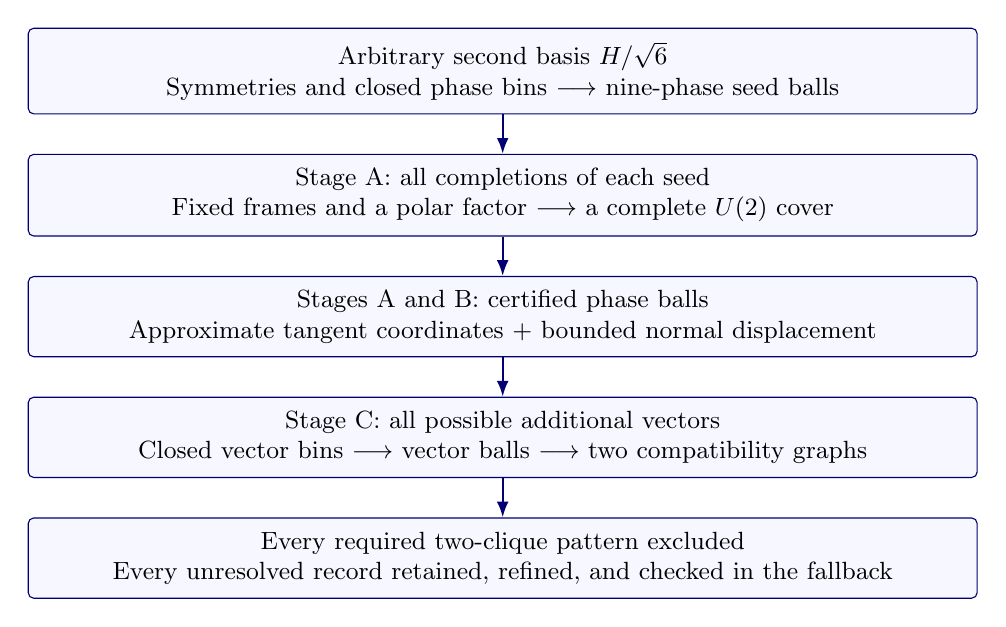
\begin{tikzpicture}[node distance=5mm,
 box/.style={draw=blue!45!black,rounded corners=2pt,fill=blue!3,
 text width=11.7cm,align=center,inner sep=5pt,font=\small},
 arr/.style={-{Latex[length=2mm]},thick,blue!45!black}]
\node[box] (seed) {Arbitrary second basis $H/\sqrt6$\\
Symmetries and closed phase bins $\longrightarrow$ nine-phase seed balls};
\node[box,below=of seed] (polar) {Stage A: all completions of each seed\\
Fixed frames and a polar factor $\longrightarrow$ a complete $U(2)$ cover};
\node[box,below=of polar] (phase) {Stages A and B: certified phase balls\\
Approximate tangent coordinates + bounded normal displacement};
\node[box,below=of phase] (graph) {Stage C: all possible additional vectors\\
Closed vector bins $\longrightarrow$ vector balls $\longrightarrow$ two compatibility graphs};
\node[box,below=of graph] (end) {Every required two-clique pattern excluded\\
Every unresolved record retained, refined, and checked in the fallback};
\draw[arr] (seed)--(polar);\draw[arr] (polar)--(phase);
\draw[arr] (phase)--(graph);\draw[arr] (graph)--(end);
\end{tikzpicture}
\end{document}
